% Generated by tools/kpi/slides.py from docs/evidence/open5gs-kpi/20261001-124845Z — do not edit by hand.
\documentclass[aspectratio=169,11pt]{beamer}
\usepackage[utf8]{inputenc}
\usepackage[T1]{fontenc}
\usepackage{lmodern}
\usepackage{helvet}
\renewcommand{\familydefault}{\sfdefault}
\usepackage{booktabs}
\usepackage{graphicx}
\usepackage{tikz}
\usetheme{Madrid}
\usefonttheme{professionalfonts}
\setbeamertemplate{navigation symbols}{}
\definecolor{brandDark}{HTML}{16324F}
\definecolor{brandMid}{HTML}{2E6E8E}
\definecolor{brandAccent}{HTML}{C7601F}
\definecolor{brandLight}{HTML}{EDF2F6}
\definecolor{okGreen}{HTML}{2C6E49}
\definecolor{softGrey}{HTML}{5A6570}
\setbeamercolor{structure}{fg=brandDark}
\setbeamercolor{palette primary}{bg=brandDark,fg=white}
\setbeamercolor{palette secondary}{bg=brandMid,fg=white}
\setbeamercolor{frametitle}{bg=brandDark,fg=white}
\setbeamercolor{block title}{bg=brandMid,fg=white}
\setbeamercolor{block body}{bg=brandLight,fg=black}
\setbeamercolor{itemize item}{fg=brandAccent}
\setbeamerfont{frametitle}{size=\large,series=\bfseries}
\setbeamerfont{block title}{size=\small,series=\bfseries}
\setbeamertemplate{itemize item}{\textbullet}
\setlength{\leftmargini}{1.4em}
% Footer carries the AI-use acknowledgement, as required.
\setbeamertemplate{footline}{%
  \hbox{%
  \begin{beamercolorbox}[wd=.30\paperwidth,ht=2.4ex,dp=1.1ex,left,leftskip=1ex]{palette primary}%
    \tiny Team 23UG005 \textbullet\ Panel 4%
  \end{beamercolorbox}%
  \begin{beamercolorbox}[wd=.52\paperwidth,ht=2.4ex,dp=1.1ex,center]{palette secondary}%
    \tiny Prepared in LaTeX Beamer; drafting assisted by an AI tool (Claude)%
  \end{beamercolorbox}%
  \begin{beamercolorbox}[wd=.18\paperwidth,ht=2.4ex,dp=1.1ex,right,rightskip=1ex]{palette primary}%
    \tiny \insertframenumber\,/\,\inserttotalframenumber%
  \end{beamercolorbox}}%
}
\begin{document}

\begin{frame}[plain]
  \begin{center}
    
\includegraphics[height=11mm]{assets/logo2.jpeg}\\[2mm]
    {\color{brandDark}\Large\bfseries Phase 2b --- Per-Slice KPIs on a 100-UE, Three-Slice 5G Core\par}
    \vspace{2mm}
    {\color{brandAccent}\small\bfseries Open5GS v2.8.0 + UERANSIM v3.3.0, measured on the running system\par}
    \vspace{1mm}
    {\color{softGrey}\footnotesize Team ID: 23UG005 \quad\textbullet\quad Panel No.\ 4 \quad\textbullet\quad KPI run 20261001-124845Z\par}
    \vspace{4mm}
    {\footnotesize Anvita Arasavilli \quad Janhavi Nilesh Parate \quad Keerthi Devarajan Anuradha \quad Mukkara Rithvik Reddy\par}
  \end{center}
\end{frame}

\begin{frame}{The ask: 100 UEs in three classes, a KPI per class}
  \begin{columns}[T]
    \column{0.48\textwidth}
    \begin{block}{From the guide's minutes}
      \small
      \begin{itemize}
        \item 10 time-sensitive UEs \textrightarrow\ \textbf{URLLC}, judged on latency
        \item 20 bandwidth UEs \textrightarrow\ \textbf{eMBB}, judged on throughput
        \item 70 IoT UEs sending 10 bytes periodically \textrightarrow\ \textbf{mMTC}
        \item KPIs compared with industry values
        \item Excel report of KPIs at all instances, varying one parameter
      \end{itemize}
    \end{block}
    \column{0.48\textwidth}
    \begin{block}{Assumptions (team KPI notes)}
      \small
      \begin{itemize}
        \item Industry-standard values are used only as benchmarks
        \item Open5GS and UERANSIM, not an industry-grade deployment
        \item In the 5G research lab, industry values can be used
      \end{itemize}
    \end{block}
  \end{columns}
\end{frame}

\begin{frame}{Topology: a dedicated user plane per slice, shared control plane}
  \footnotesize
  \begin{tabular}{@{}llll@{}}
    \toprule
    & \textbf{eMBB} & \textbf{URLLC} & \textbf{mMTC} \\
    \midrule
    S-NSSAI & SST 1 / 010203 & SST 2 / 112233 & SST 3 / 334455 \\
    UEs & 20 & 10 & 70 \\
    5QI \textbullet\ session AMBR & 9 \textbullet\ 200 Mbps & 82 \textbullet\ 20 Mbps & 9 \textbullet\ 1 Mbps \\
    gNB, UPF, data network & own & own & own \\
    Traffic & TCP bulk download & 64 B every 20 ms & 10 B every 10 s \\
    \bottomrule
  \end{tabular}

  \vspace{3mm}
  \begin{block}{How the KPIs are measured}
    \footnotesize Every packet leaves from the device's own PDU-session address and crosses its slice's gNB and UPF.
    Latency is one-way, device to data network: sender and receiver share one monotonic clock (same kernel),
    so no clock synchronisation error. Loss from per-device sequence numbers.
  \end{block}
\end{frame}

\begin{frame}{KPIs and targets (team notes), with industry benchmarks}
  \scriptsize
  \resizebox{\textwidth}{!}{%
  \begin{tabular}{@{}lllll@{}}
    \toprule
    \textbf{Slice} & \textbf{KPI} & \textbf{Project target} & \textbf{Research target} & \textbf{Industry benchmark} \\
    \midrule
URLLC & End-to-end user-plane latency, mean & 10 ms & 2 ms & 1 ms {\tiny(ITU-R M.2410)} \\
URLLC & Latency, 95th percentile & 10 ms & --- & 10 ms {\tiny(3GPP TS 23.501 Table 5.7.4-1)} \\
URLLC & Latency, 99th percentile & 10 ms & --- & 10 ms {\tiny(3GPP TS 23.501 Table 5.7.4-1)} \\
URLLC & Packet loss & 0.01\,\% & --- & 0.01\,\% {\tiny(3GPP TS 23.501 Table 5.7.4-1)} \\
eMBB & 5th-percentile user throughput, downlink & 50 Mbps & --- & 100 Mbps {\tiny(ITU-R M.2410)} \\
eMBB & Aggregate downlink throughput of the slice & --- & 500 Mbps & 550 Mbps {\tiny(Research papers)} \\
mMTC & UE registration success rate & 99\,\% & --- & --- {\tiny(3GPP TR 38.913)} \\
mMTC & Report loss & --- & 0.1\,\% & 0.1\,\% {\tiny(Research papers)} \\
mMTC & Report latency, 99th percentile & 10000 ms & --- & 10000 ms {\tiny(3GPP TR 38.913)} \\
    \bottomrule
  \end{tabular}}

  \vspace{2mm}
  {\scriptsize\color{softGrey} Score per KPI: 1 if met, else the fraction of the way to the target. Slice score: weighted sum (weights provisional).}
\end{frame}

\begin{frame}{Result: all three slices served at once (150 s, 20 eMBB UEs downloading)}
  \scriptsize
  \begin{tabular}{@{}lllllll@{}}
    \toprule
    \textbf{Slice} & \textbf{KPI} & \textbf{Measured} & \textbf{Target} & \textbf{Benchmark} & \textbf{Result} & \textbf{Score} \\
    \midrule
URLLC & End-to-end user-plane latency, mean & 3.93 ms & 10 ms & 1 ms & \textcolor{okGreen}{\textbf{met}} & 1.00 \\
URLLC & Latency, 95th percentile & 11.44 ms & 10 ms & 10 ms & \textcolor{brandAccent}{\textbf{missed}} & 0.87 \\
URLLC & Latency, 99th percentile & 22.04 ms & 10 ms & 10 ms & \textcolor{brandAccent}{\textbf{missed}} & 0.45 \\
URLLC & Packet loss & 0\,\% & 0.01\,\% & 0.01\,\% & \textcolor{okGreen}{\textbf{met}} & 1.00 \\
eMBB & 5th-percentile user throughput, downlink & 10.83 Mbps & 50 Mbps & 100 Mbps & \textcolor{brandAccent}{\textbf{missed}} & 0.22 \\
eMBB & Aggregate downlink throughput of the slice & 299.3 Mbps & 500 Mbps & 550 Mbps & \textcolor{brandAccent}{\textbf{missed}} & 0.60 \\
mMTC & UE registration success rate & 100\,\% & 99\,\% & --- & \textcolor{okGreen}{\textbf{met}} & 1.00 \\
mMTC & Report loss & 0\,\% & 0.1\,\% & 0.1\,\% & \textcolor{okGreen}{\textbf{met}} & 1.00 \\
mMTC & Report latency, 99th percentile & 18.0 ms & 10000 ms & 10000 ms & \textcolor{okGreen}{\textbf{met}} & 1.00 \\
    \bottomrule
  \end{tabular}

  \vspace{2mm}
  \footnotesize Slice scores: \textbf{URLLC 0.90} \textbullet\ \textbf{eMBB 0.37} \textbullet\ \textbf{mMTC 1.00} \textbullet\ overall 0.76
\end{frame}

\begin{frame}{Sweep 1: eMBB load (devices downloading at once)}
  \begin{columns}[T]
    \column{0.5\textwidth}
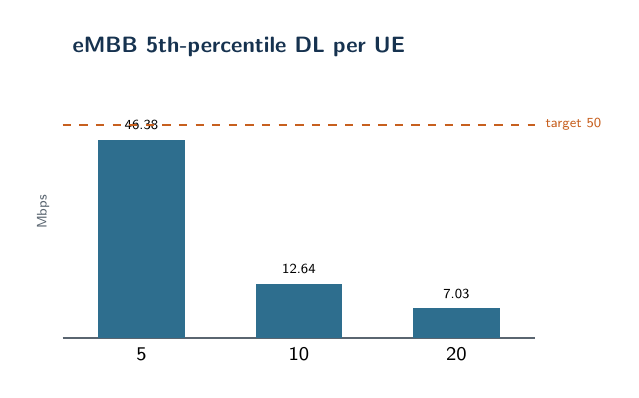
\begin{tikzpicture}[font=\scriptsize]
\node[anchor=south west,font=\footnotesize\bfseries,text=brandDark] at (0,3.45) {eMBB 5th-percentile DL per UE};
\draw[softGrey] (0,0) -- (6.00,0);
\fill[brandMid] (0.45,0) rectangle (1.55,2.52);
\node[above,font=\tiny] at (1.00,2.52) {46.38};
\node[below] at (1.00,0) {5};
\fill[brandMid] (2.45,0) rectangle (3.55,0.69);
\node[above,font=\tiny] at (3.00,0.69) {12.64};
\node[below] at (3.00,0) {10};
\fill[brandMid] (4.45,0) rectangle (5.55,0.38);
\node[above,font=\tiny] at (5.00,0.38) {7.03};
\node[below] at (5.00,0) {20};
\draw[brandAccent,thick,dashed] (0,2.71) -- (6.00,2.71) node[right,font=\tiny,text=brandAccent] {target 50};
\node[rotate=90,font=\tiny,text=softGrey] at (-0.25,1.60) {Mbps};
\end{tikzpicture}
    \column{0.5\textwidth}
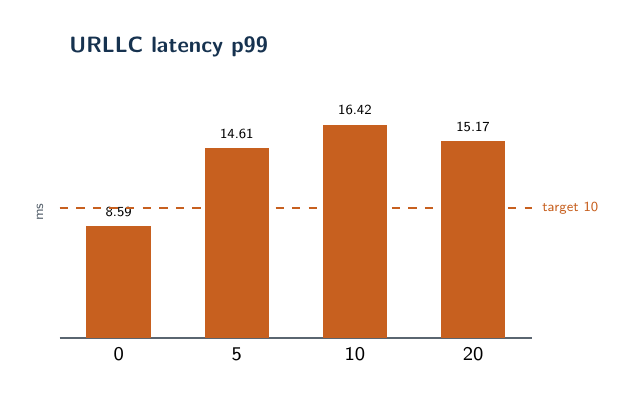
\begin{tikzpicture}[font=\scriptsize]
\node[anchor=south west,font=\footnotesize\bfseries,text=brandDark] at (0,3.45) {URLLC latency p99};
\draw[softGrey] (0,0) -- (6.00,0);
\fill[brandAccent] (0.34,0) rectangle (1.16,1.42);
\node[above,font=\tiny] at (0.75,1.42) {8.59};
\node[below] at (0.75,0) {0};
\fill[brandAccent] (1.84,0) rectangle (2.66,2.41);
\node[above,font=\tiny] at (2.25,2.41) {14.61};
\node[below] at (2.25,0) {5};
\fill[brandAccent] (3.34,0) rectangle (4.16,2.71);
\node[above,font=\tiny] at (3.75,2.71) {16.42};
\node[below] at (3.75,0) {10};
\fill[brandAccent] (4.84,0) rectangle (5.66,2.50);
\node[above,font=\tiny] at (5.25,2.50) {15.17};
\node[below] at (5.25,0) {20};
\draw[brandAccent,thick,dashed] (0,1.65) -- (6.00,1.65) node[right,font=\tiny,text=brandAccent] {target 10};
\node[rotate=90,font=\tiny,text=softGrey] at (-0.25,1.60) {ms};
\end{tikzpicture}
  \end{columns}
  \vspace{2mm}
  \footnotesize With 5 devices the 5th percentile is close to the 50 Mbps target; with 20 it falls to 7.03 Mbps.
  The laptop delivers about 275.1--357.7 Mbps in total, so 50 Mbps for each of 20 UEs (1 Gbps) is out of reach here.
  eMBB load also pushes URLLC's tail past 10 ms: the slices share one CPU.
\end{frame}

\begin{frame}{Sweep 2: more IoT devices (``later increase the UEs'')}
  \begin{columns}[T]
    \column{0.5\textwidth}
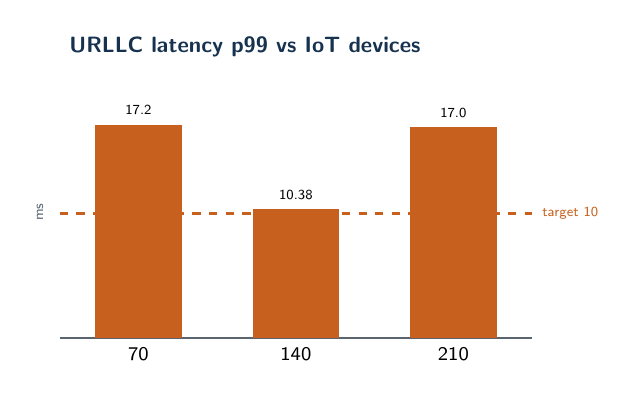
\begin{tikzpicture}[font=\scriptsize]
\node[anchor=south west,font=\footnotesize\bfseries,text=brandDark] at (0,3.45) {URLLC latency p99 vs IoT devices};
\draw[softGrey] (0,0) -- (6.00,0);
\fill[brandAccent] (0.45,0) rectangle (1.55,2.71);
\node[above,font=\tiny] at (1.00,2.71) {17.2};
\node[below] at (1.00,0) {70};
\fill[brandAccent] (2.45,0) rectangle (3.55,1.64);
\node[above,font=\tiny] at (3.00,1.64) {10.38};
\node[below] at (3.00,0) {140};
\fill[brandAccent] (4.45,0) rectangle (5.55,2.68);
\node[above,font=\tiny] at (5.00,2.68) {17.0};
\node[below] at (5.00,0) {210};
\draw[brandAccent,thick,dashed] (0,1.58) -- (6.00,1.58) node[right,font=\tiny,text=brandAccent] {target 10};
\node[rotate=90,font=\tiny,text=softGrey] at (-0.25,1.60) {ms};
\end{tikzpicture}
    \column{0.5\textwidth}
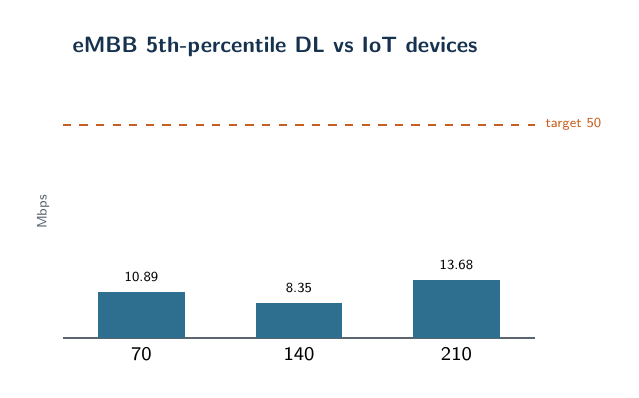
\begin{tikzpicture}[font=\scriptsize]
\node[anchor=south west,font=\footnotesize\bfseries,text=brandDark] at (0,3.45) {eMBB 5th-percentile DL vs IoT devices};
\draw[softGrey] (0,0) -- (6.00,0);
\fill[brandMid] (0.45,0) rectangle (1.55,0.59);
\node[above,font=\tiny] at (1.00,0.59) {10.89};
\node[below] at (1.00,0) {70};
\fill[brandMid] (2.45,0) rectangle (3.55,0.45);
\node[above,font=\tiny] at (3.00,0.45) {8.35};
\node[below] at (3.00,0) {140};
\fill[brandMid] (4.45,0) rectangle (5.55,0.74);
\node[above,font=\tiny] at (5.00,0.74) {13.68};
\node[below] at (5.00,0) {210};
\draw[brandAccent,thick,dashed] (0,2.71) -- (6.00,2.71) node[right,font=\tiny,text=brandAccent] {target 50};
\node[rotate=90,font=\tiny,text=softGrey] at (-0.25,1.60) {Mbps};
\end{tikzpicture}
  \end{columns}
  \vspace{2mm}
  \footnotesize Up to 210 IoT devices (240 UEs): every device registered, no report was lost.
  Sweep 3, reporting interval 1--30 s: mMTC loss 0 at every interval.
  Across all 9 instances with 20 eMBB UEs and identical settings, eMBB aggregate ranged 254.6--454.9 Mbps:
  host conditions on this laptop move eMBB more than IoT scale does --- repeat runs on the lab machine.
\end{frame}

\begin{frame}{Findings, and what this setup cannot show}
  \begin{columns}[T]
    \column{0.5\textwidth}
    \begin{block}{Findings}
      \footnotesize
      \begin{itemize}
        \item URLLC mean latency 3.93 ms meets 10 ms; its p99 (22.04 ms) does not under eMBB load
        \item eMBB is capped by the laptop, not the slice design: with 20 UEs the 5th percentile never exceeded 13.68 Mbps
        \item mMTC: 100\% registration, 0 loss, up to 240 UEs
        \item Bugs found on the way: simulator clock, three start-up races, gNB never reconnecting, a deploy reporting success it never applied --- all fixed
      \end{itemize}
    \end{block}
    \column{0.5\textwidth}
    \begin{block}{Not measurable with a simulated RAN}
      \footnotesize
      \begin{itemize}
        \item Radio-only latency (ITU's 1 ms), spectral efficiency
        \item Coverage, mobility, devices per km$^2$
        \item IoT battery life and real sleep modes
      \end{itemize}
    \end{block}
  \end{columns}
\end{frame}

\begin{frame}{To confirm with the guide, and next}
  \begin{columns}[T]
    \column{0.5\textwidth}
    \begin{block}{Provisional choices}
      \footnotesize
      \begin{itemize}
        \item Traffic: URLLC 64 B / 20 ms; IoT 10 B every 10 s
        \item KPI weights and the overall score
        \item The two eMBB targets contradict (1 Gbps vs 500 Mbps)
        \item Sweep parameters
      \end{itemize}
    \end{block}
    \column{0.5\textwidth}
    \begin{block}{Next}
      \footnotesize
      \begin{itemize}
        \item Orchestrator: priority within URLLC, deciding the slices, allocation from these KPIs
        \item Re-run on the lab's bare-metal machine
        \item Fault diagnosis (later phase)
      \end{itemize}
    \end{block}
  \end{columns}
\end{frame}

\end{document}
